\documentclass[12pt]{beamer}
\graphicspath{{Imagenes/}{../Imagenes/}}
\usepackage[utf8]{inputenc}
\usepackage[spanish]{babel}
\usepackage{etex}
\usepackage{amsmath}
\usepackage{amsthm}
\usepackage{booktabs}
\usepackage{tabulary}
\usepackage{nccmath}
\usepackage{multicol}
\usepackage{multirow}
\usepackage{graphicx}
\usepackage{tikz}
\usetikzlibrary{patterns}
\usetikzlibrary{decorations.markings}
% Introduce a new counter for counting the nodes needed for circling
\newcounter{nodecount}
% Command for making a new node and naming it according to the nodecount counter
\newcommand\tabnode[1]{\addtocounter{nodecount}{1} \tikz \node (\arabic{nodecount}) {#1};}
% Some options common to all the nodes and paths
\tikzstyle{every picture}+=[remember picture,baseline]
\tikzstyle{every node}+=[inner sep=0pt,anchor=base,
minimum width=2.2cm,align=center,text depth=.15ex,outer sep=1.5pt]
\tikzstyle{every path}+=[thick, rounded corners]
\usepackage{color}
\usepackage{listings}
\renewcommand*{\multirowsetup}{\centering}
\usetikzlibrary{arrows}
\usepackage{color}
\usepackage{listings}
\usepackage{hyperref}
\renewcommand {\arraystretch}{1.5}
\mode<presentation>
{
  \usetheme{Warsaw}  
  %\usetheme{CambridgeUS}
  %\setbeamercovered{transparent}
  % or whatever (possibly just delete it)
  
  \setbeamertemplate{headline}{}
  %\useoutertheme{infolines}
  \useoutertheme{default}
  \setbeamercovered{invisible}
  % or whatever (possibly just delete it)
}

\usepackage{listings}
\lstset{ %
language=Python,                % choose the language of the code
basicstyle=\small,       % the size of the fonts that are used for the code
numbers=left,                   % where to put the line-numbers
numberstyle=\small,      % the size of the fonts that are used for the line-numbers
stepnumber=1,                   % the step between two line-numbers. If it is 1 each line will be numbered
numbersep=5pt,                  % how far the line-numbers are from the code
backgroundcolor=\color{white},  % choose the background color. You must add \usepackage{color}
showspaces=false,               % show spaces adding particular underscores
showstringspaces=false,         % underline spaces within strings
showtabs=false,                 % show tabs within strings adding particular underscores
frame=single,   		% adds a frame around the code
tabsize=2,  		% sets default tabsize to 2 spaces
captionpos=b,   		% sets the caption-position to bottom
breaklines=true,    	% sets automatic line breaking
breakatwhitespace=false,    % sets if automatic breaks should only happen at whitespace
escapeinside={\%},          % if you want to add a comment within your code
stringstyle =\color{magenta},
keywordstyle = \color{blue},
commentstyle = \color{green},
identifierstyle = \color{red}
}
\title{Ecuaciones diferenciales ordinarias}
\subtitle{Curso de Física Computacional}
\author[]{M. en C. Gustavo Contreras Mayén}
\begin{document}
\maketitle
\fontsize{14}{14}\selectfont
\spanishdecimal{.}
\begin{frame}{Contenido}
\tableofcontents[pausesections]
\end{frame}
\section{Introducción}
\begin{frame}
\frametitle{Introducción.}
Las ecuaciones diferenciales tienen importancia fundamental en las aplicaciones, ya que muchas leyes y relaciones físicas pueden expresarse matemáticamente de esta forma.
\\
\medskip
En particular, el estudio de problemas de equilibrio de sistemas continuos se encuentra dentro de este contexto.
\end{frame}
\subsection{Definiciones importantes para recordar}
\begin{frame}
\frametitle{Definiciones importantes}
\begin{block}{Aviso de consideración}
	No sería mala idea hacer un repaso en casa sobre estas definiciones y los métodos analíticos de solución de las	 \textit{Ecuaciones Diferenciales Ordinarias} EDO.
\end{block}
\end{frame}
\begin{frame}
\frametitle{Ecuación diferencial}
Esta ecuación relaciona dos o más variables en términos de derivadas o diferenciales.
\\
\fontsize{12}{12}\selectfont
\begin{eqnarray*}
	\dfrac{dy}{dx} & = & \cos x \\
	\dfrac{d^{2} y}{dx^{2}} & = &  \cos x \\
	( x^{2} + y^{2} ) dx + 2 xy dy & = & 0 \\
	\left[ \dfrac{x^{2} w}{dx^{2}} \right]^{3} - xy \dfrac{dw}{dx} & = & 0 
\end{eqnarray*}
\end{frame}
\begin{frame}
\frametitle{Ecuaciones diferenciales ordinarias (EDO) y parciales}
Si en una ecuación diferencial hay una sola variable independiente, las derivadas son totales y se le llama \textit{ecuación ordinaria}.
\\
\medskip
Si en la ecuación hay dos o más variables independientes, las derivadas serán parciales y se le llama \textit{ecuación parcial}.
\[ \dfrac{\partial^{2} V}{\partial x^{2}} + \dfrac{\partial^{2} V}{\partial y^{2}} = 0\]
\end{frame}
\begin{frame}
\frametitle{Orden de una ecuación diferencial}
Es la derivada de mayor orden que aparece en la ecuación.
\end{frame}
\begin{frame}
\frametitle{Grado de una ecuación diferencial}
Es el grado \textit{algebraico} de la derivada de mayor orden que aparece en la ecuación.
\end{frame}
\begin{frame}
\frametitle{Ecuación diferencial lineal}
Una ecuación diferencial es lineal si en ella no aparecen potencias de la variable dependiente y sus derivadas, ni productos de la variable dependiente por sus derivadas o productos entre derivadas.
\end{frame}
\begin{frame}
\frametitle{Solución de una ecuación diferencial}
Es cualquier relación funcional que no incluya derivadas o integrales de funciones desconocidas y que implique a la propia ecuación diferencial, en el sentido de que la verifique por sustitución directa.
\end{frame}
\begin{frame}
\frametitle{Ecuación y condiciones homogéneas}
Una ecuación o condición es homogénea si, cuando es satisfecha por una función particular $y(x)$, también es satisfecha por $cy(x)$, donde $c$ es una constante arbitraria.
\end{frame}
\begin{frame}
\frametitle{Solución de una ecuación diferencial}
Sea una ecuación diferencial ordinaria de orden $n$ y cualquier grado, cuya forma más general es:
\[F(x, y, y', y'', \ldots, y^{(n)}) = 0\]
Se establece del cálculo que en su solución general deben de aparecer $n$ constantes arbitrarias. Entonces puede aceptarse como solución general:
\[G(x,y,c_{1},c_{2}, \ldots, c_{n}) = 0\]
\end{frame}
\begin{frame}[fragile]
\frametitle{Solución de una EDO}
\begin{tikzpicture}[font=\small]
	\draw [->] (0,0) -- (7,0);
	\draw [->] (0,0) -- node [near end, left] {y} (0,5);
	\draw (1,1) .. controls (2.5,2.5) and (4,3) .. (6,3);
	\draw (1,2) .. controls (2.5,3.5) and (4,4) .. (6,4);
	\draw (1,0.2) .. controls (2.5,1.7) and (4,2.2) .. (6,2.2);
	\draw (7.3,-0.1) node {x};
	\draw (7.2,2.2) node {$G_{1}=0$};
	\draw (7.2,4.2) node {$G_{2}=0$};
	\draw (7.2,3.2) node {$G_{3}=0$};
\end{tikzpicture}
\end{frame}
\begin{frame}
\frametitle{Ejemplo}
Gráficamente esta ecuación representa a una familia de curvas planas, cada una de ellas obtenidas para valores particulares de las $n$ constantes $c_{1}, c_{2}, \ldots, c_{n}$
\end{frame}
\begin{frame}
\frametitle{Tipos de problemas}
Dependiendo de cómo se establezcan estas condiciones, se distinguen dos tipos de problemas los llamados {\color{red}\textit{de valores iniciales}} y los {\color{red}\textit{de valores en la frontera}}.
\end{frame}
\begin{frame}
\frametitle{Problemas de valores iniciales}
Está gobernado por una ecuación diferencial de orden $n$ y un conjunto de $n$ condiciones independientes, todas ellas válidas para el mismo punto inicial.
\\
\medskip
Si la ecuación diferencial que define el problema es del tipo de la EDO con la que iniciamos y $x=a$ es el punto inicial, puede aceptarse que las $n$ condiciones independientes son:
\end{frame}
\begin{frame}
\frametitle{$n$ condiciones independientes}
\begin{eqnarray*}
	y(a) & = & y_{0} \\
	y'(a) & = & y'_{0} \\
	y''(a) & = & y''_{0} \\
	\vdots \\
	y^{n}(a) & = & y^{n}_{0}
\end{eqnarray*}
Y se tratará de obtener una solución particular de la EDO inicial que verifique las condiciones iniciales, como se presenta en la siguiente figura:
\end{frame}
\begin{frame}[fragile]
\frametitle{Solución de una EDO con condiciones inciales}
\begin{tikzpicture}[font=\small]
	\draw [->] (0,0) -- (7,0);
	\draw [->] (0,0) -- node [near end, left] {y} (0,5);
	\draw (1,2) .. controls (2.5,3.5) and (4,4) .. (6,4);
	\draw (7.3,-0.1) node {x};
	\draw (7.2,4.2) node {$g(x,y)=0$};
	\draw [dashed] (1.5,0) -- (1.5,2.4);
	\draw (1.3,-0.2) node {x=a};
\end{tikzpicture}
\end{frame}
\begin{frame}
\frametitle{Problemas de valores en la frontera}
Se deben de establecer condiciones de frontera en todos y cada uno de los puntos que constituyen la frontera del dominio de soluciones del problema.
\\
\medskip
En particular, en el espacio de una dimensión, hay dos puntos frontera, por ejemplo $x=a$ y $x=b$ si el dominio de soluciones es el intervalo cerrado $a \leq x \leq b$
\end{frame}
\begin{frame}[fragile]
\frametitle{Solución de una EDO con condiciones de frontera}
\begin{tikzpicture}[font=\small]
	\draw [->] (0,0) -- (7,0);
	\draw [->] (0,0) -- node [near end, left] {y} (0,5);
	\draw (1,2) .. controls (2.5,3.5) and (4,4) .. (6,4);
	\draw (7.3,-0.1) node {x};
	\draw (7.2,4.2) node {$g(x,y)=0$};
	\draw [dashed] (1.5,0) -- (1.5,2.4);
	\draw (1.3,-0.2) node {x=a};
	\draw [dashed] (5.2,0) -- (5.2,4);
	\draw (5,-0.2) node {x=b};
\end{tikzpicture}
\end{frame}
\begin{frame}
\frametitle{Estrategia de solución}
Básicamente la solución numérica de las ecuaciones diferenciales consiste en sustituir el dominio continuo de soluciones por uno discreto formado por puntos aislados igualmente espaciados entre sí.
\end{frame}
\begin{frame}
\frametitle{Problema de valores iniciales}
El dominio de definición de soluciones $x \geq a$  se sustituye por el conjunto infinito numerable de puntos:
\begin{eqnarray*}
	x_{0} & = & a \\
	x_{1} & = & x_{0} + h \\
	x_{2} & = & x_{0} + 2h \\
	x_{3} & = & x_{0} + 3h \\
	\ldots
\end{eqnarray*}
\end{frame}
\begin{frame}[fragile]
\frametitle{Valores inciales}
\begin{tikzpicture}[font=\small]
	\draw [->] (0,0) -- (7,0);
	\draw [->] (0,0) -- node [near end, left] {y} (0,5);
	\draw (1,2) .. controls (2.5,3.5) and (4,4) .. (6,4);
	\draw (7.3,-0.1) node {x};
	\draw (7.2,4.2) node {$g(x,y)=0$};
	\draw [dashed] (1.5,0) -- (1.5,2.4);
	\draw (1.3,-0.2) node {$x_{0}=a$};
	\draw [dashed] (2.3,0) -- (2.3,3.15);
	\draw (2.3,-0.2) node {$x_{1}$};
	\draw [dashed] (3.3,0) -- (3.3,3.6);
	\draw (3.3,-0.2) node {$x_{2}$};
	\draw [dashed] (4.3,0) -- (4.3,3.85);
	\draw (4.3,-0.2) node {$x_{3}$};
	\draw (5.3,-0.2) node {$\ldots$};
\end{tikzpicture}
\end{frame}
\begin{frame}
\frametitle{Problema de valores en la frontera}
Se sustituye el intervalo $a \leq x \leq b $ por el conjunto finito de puntos:
\begin{eqnarray*}
	x_{0} & = & a \\
	x_{1} & = & x_{0} + h \\
	x_{2} & = & x_{0} + 2h \\
	x_{3} & = & x_{0} + 3h \\
	\ldots \\
	x_{n} & = & x_{0} + nh = b
\end{eqnarray*}
\end{frame}
\begin{frame}[fragile]
\frametitle{Valores en la frontera}
\begin{tikzpicture}[font=\small]
	\draw [->] (0,0) -- (7,0);
	\draw [->] (0,0) -- node [near end, left] {y} (0,5);
	\draw (1,2) .. controls (2.5,3.5) and (4,4) .. (6,4);
	\draw (7.3,-0.1) node {x};
	\draw (7.2,4.2) node {$g(x,y)=0$};
	\draw [dashed] (1.5,0) -- (1.5,2.4);
	\draw (1.3,-0.2) node {$x_{0}=a$};
	\draw [dashed] (2.3,0) -- (2.3,3.15);
	\draw (2.3,-0.2) node {$x_{1}$};
	\draw [dashed] (3.3,0) -- (3.3,3.6);
	\draw (3.3,-0.2) node {$x_{2}$};
	\draw [dashed] (4.3,0) -- (4.3,3.85);
	\draw (4.3,-0.2) node {$x_{3}$};
	\draw (5.1,-0.2) node {$\ldots$};
	\draw [dashed] (5.9,0) -- (5.9,4);
	\draw (6,-0.2) node {$x_{n}=b$};
\end{tikzpicture}
\end{frame}
\begin{frame}
\frametitle{Nuestra tarea}
Habiéndose discretizado el problema continuo, se tratará de obtener la solución para los puntos considerados, esto se resuelve en general, sustituyendo las derivadas que aparezcan en la ecuación diferencial y en sus condiciones iniciales o de frontera, por fórmulas numéricas de derivación que proporcionen una aproximación a a las derivadas o tratando de integrar la ecuación, reemplazando el proceso de integración por una fórmula numérica que se aproxime a la integral.
\end{frame}
\section{Problemas de valores iniciales}
\begin{frame}
\frametitle{Problemas de valores iniciales}
Debemos de resovler
\[ y' = F(x,y)\]
con la condición auxiliar $y(a) = \alpha$
\end{frame}
\begin{frame}
\frametitle{Forma general de una EDO de 1er. orden}
La forma general de una ecuación diferencial de primer orden (1-EDO) es
\[ y' = f(x,y) \]
donde $y' = dy/dx$ y $f(x,y)$ es una función dada.
\\
\bigskip
La solución de esta ecuación incluye una constante arbitraria (la constante de integración); para hallar esa constante, debemos conocer un punto en la curva solución, esto es, $y$ debe de especificarse para algún valor de $x$, $x=a$. Entonces, escribimos, la condición auxiliar $y(a) = \alpha$
\end{frame}
\begin{frame}
Una ecuación diferencial de orden $n$
\[y^{(n)} = f(x,y,y',\ldots,y^{(n-1)})\]
se puede transformar en un conjunto de $n$ ecuaciones diferenciales de primer orden; usemos la notación
\begin{eqnarray*}
y_{0} &=& y \\
y_{1} &=& y' \\
y_{2} &=& y'' \\
\ldots \\
y_{n-1} &=& y^{(n-1)}
\end{eqnarray*}
\end{frame}
\begin{frame}
Las ecuaciones 1-EDO equivalentes son:
\begin{eqnarray*}
y'_{0} &=& y_{1} \\
y'_{1} &=& y_{2} \\
y'_{2} &=& y_{3} \\
\ldots \\
y'_{n} &=& f(x,y_{0},y_{1},\ldots,y_{n-1})
\end{eqnarray*}
\end{frame}
\begin{frame}
La solución ahora requiere de $n$ condiciones auxiliares; si esas condiciones se especifican para el mismo valor de $x$, el problema se dice que es \emph{un problema de valores iniciales}.
\\
\medskip
Las condiciones auxiliares, se llaman \emph{condiciones iniciales}, que tienen la forma:
\[ y_{0}(a) = \alpha_{0} \hspace{1cm} y_{1}(a) = \alpha_{1} \hspace{1cm} \ldots \hspace{1cm} y_{n-1}(a) = \alpha_{n-1}\]
\end{frame}
\begin{frame}
Si $y_{i}$ se especifica para diferentes valores de $x$, el problema se llama \emph{problema con condiciones de frontera}, por ejemplo:
\[ y'' = -y \hspace{1cm} y(0)=1 \hspace{1cm} y'(0) = 0\]
es un problema de condiciones iniciales, ya que ambas condiciones están definidas en la solución para $x=0$, en cambio
\[ y'' = -y \hspace{1cm} y(0)=1 \hspace{1cm} y'(\pi) = 0\]
es un problema con condiciones de frontera, ya que las dos condiciones se cumplen para diferentes valores de $x$.
\end{frame}
\begin{frame}
\frametitle{Notación usada para el tema EDO}
Se usará de manera continua y por conveniencia, la notación vectorial, que nos permitirá manejar conjuntos de 1-EDO de una manera más clara, de tal manera que podremos expresar:
\[ \mathbf{y}' = \mathbf{F}(x,\mathbf{y}) \hspace{1.3cm} \mathbf{y}(a) = \alpha\]
\[ \mathbf{F}(x,\mathbf{y}) = \left[ \begin{matrix}
y_{1} \\
y_{2} \\
\ldots \\
f(x,\mathbf{y}
\end{matrix} \right] \]
\end{frame}
\section{Método de la Serie de Taylor}
\begin{frame}
\frametitle{Método de la Serie de Taylor}
El método de la Serie de Taylor es sencillo conceptualmente y con una mayor precisión.
\\
\medskip
Se basa en la serie de Taylor truncada para $y$ alrededor de $x$:
\[ \begin{split}
y(x+h) & \simeq y(x) + y'(x) h +  \dfrac{1}{2!} y''(x)h^{2} + \dfrac{1}{3!} y'''(x) h^{3} + \\
& + \ldots + \dfrac{1}{m!} y^{(m)}(x) h^{m} \end{split} \]
\end{frame}
\begin{frame}
La fórmula anterior predice el valor de $y$ en $x+h$ con la información disponible de $x$, y es también una fórmula de integración numérica.
\\
\medskip
El último término en la serie determina el orden de integración, en el ejemplo el orden de integración, es $m$.
\end{frame}
\begin{frame}
\frametitle{Error de truncamiento}
El error debido al truncamiento, es:
\[ E = \dfrac{1}{(m+1)!} y^{(m+1)} (\xi) h^{m+1}, \hspace{1cm} x<\xi<x+h \]
\end{frame}
\begin{frame}
Usando la aproximación por diferencias finitas
\[ y^{(m+1)} (\xi) \simeq \dfrac{y^{(m)}(x+h)-y^{(m)}(x)}{h}\]
para obtener una expresión más amigable
\[ E \simeq \dfrac{h^{m}}{(m+1)!} \left[ y^{(m)}(x+h) - y^{(m)}(x) \right]\]
la cual se puede incorporar en el algoritmo y revisar el error en cada paso de integración.
\end{frame}
\section{La función \texttt{taylor}}
\begin{frame}
\frametitle{La función \texttt{taylor}}
Vamos a construir una función que use el método de series de Taylor con un cuarto orden de integración.
\\
\medskip
Con esta función podremos manejar cualquier número de 1-EDO $y_{i} = f_{i} (x, y_{0},y_{1},\ldots)$, con $i=0,1,\ldots$
\\
\medskip
El usuario deberá de proporcionar la función \texttt{deriv} que devuelva el arreglo de $4 \times n$
\[ \mathbf{D} = 
\begin{bmatrix}
(\mathbf{y}')^{T} \\
(\mathbf{y}'')^{T} \\
(\mathbf{y}''')^{T} \\
(\mathbf{y}^{4})^{T}
\end{bmatrix} =
\begin{bmatrix}
y'_{0} & y'_{1} & \ldots & y'_{n-1} \\
y''_{0} & y''_{1} & \ldots & y''_{n-1} \\
y'''_{0} & y'''_{1} & \ldots & y'''_{n-1} \\
y^{4}_{0} & y^{4}_{1} & \ldots & y^{4}_{n-1}
\end{bmatrix} \]
La función devuelve los arreglos \texttt{X} y \texttt{Y} que contienen los valores de $x$ y de $y$ en intervalos $h$.
\end{frame}
\begin{frame}[fragile]
\begin{lstlisting}
def taylor(deriv,x,y,xAlto,h):
    X=[]
    Y=[]
    X.append(x)
    Y.append(y)
    while x<xAlto:
        h= min(h,xAlto-x)
        D= deriv(x,y)
        H= 1.0
        for j in range(4):
            H = H*h /(j+1)
            y = y + D[j]*H
        x= x+h
        X.append(x)
        Y.append(y)
    return array(X), array(Y)
\end{lstlisting}
\end{frame}
\begin{frame}
\frametitle{Rutinas para visualizar los resultados}
A continuación se presentan dos rutinas que nos ayudarán a visualizar mejor los resultados en pantalla.
\\
\medskip
Usaremos la función \texttt{imprimeSoln} para imprimir $X$ y $Y$ obtenidas de la integración numérica, la cantidad de datos, se controla con el parámetro \texttt{freq}, si \texttt{freq=5}, cada cinco pasos, se presentará el valor, si \texttt{freq=0}, el valor inicial y el final, se presentarán.
\end{frame}
\begin{frame}[fragile]
\begin{lstlisting}
def imprimeSoln(X,Y,freq):
   
   def imprimeEncabezado(n):
       print '\n x ',
       for i in range (n):
           print ' y[',i,']',
       print
    
    def imprimeLinea(x,y,n):
        print '%13.4e' %x,
        for i in range (n):
            print '%13.4e' %y[i],
            print
    m = len(Y)
\end{lstlisting}
\end{frame}
\begin{frame}[fragile]
\begin{lstlisting}
    try: n = len(Y[0])
    except TypeError: n = 1
    if freq == 0: freq = m

    imprimeEncabezado(n)
    for i in range(0,m,freq):
        imprimeLinea(X[i],Y[i],n)
    if i != m - 1: imprimeLinea(X[m - 1],Y[m - 1],n)
\end{lstlisting}
\end{frame}
\subsection{Ejemplo 1}
\begin{frame}
\frametitle{Ejemplo 1}
Dada la 1-EDO
\[ y' + 4y = x^{2} \hspace{1.5cm} y(0)=1 \]
Calcular 
\begin{enumerate}
\item $y(0.1)$ con el método de la serie de Taylor de cuarto orden, usando un paso de integración.
\item  también calcula el error estimado, compáralo con la solución exacta.
\\
\medskip
La solución analítica de la EDO es:
\[ y =  \dfrac{31}{32} \exp(-4x) + \dfrac{1}{4} x^{2} - \dfrac{1}{8} x + \dfrac{1}{32} \]
\end{enumerate}
\end{frame}
\begin{frame}
\frametitle{Solución}
La serie de Taylor que incluye el término con $h^{4}$ es
\[ y(h) = y(0) + y'(0)h + \dfrac{1}{2!} y''(0)h^{2} + \dfrac{1}{3!} y'''(0)h^{3} + \dfrac{1}{4!} y^{(4)}(0) h^{4} \]
Haciendo las derivadas
\begin{eqnarray*}
y' &=& -4y + x^{2} \\
y'' &=& -4y' + 2x = 16y - 4x^{2}+2x \\
y''' &=& 16y' - 8x + 2 = -64y + 16x^{2} - 8x + 2 \\
y^{(4)} &=& -64 y'+32x-8 = 256y - 64x^{2}+32x-8 
\end{eqnarray*}
\end{frame}
\begin{frame}
Que en $x=0$
\begin{eqnarray*}
y'(0) &=& -4(1) = -4 \\
y''(0) &=& 16(1) = 16 \\
Y'''(0) &=& -64(1) + 2 = -62 \\
y^{(4)}(0) &=& 256(1) - 8 = 248
\end{eqnarray*}
Con $h=0.1$, resulta
\[ \begin{split}
y(0.1) &= 1 + (-4)(0.1) + \dfrac{1}{2!}(16)(0.1)^{2} + \\ &+ \dfrac{1}{3!} (-62)(0.1)^{3} + \dfrac{1}{4!} (248)(0.1)^{4} \\
&= 0.670700 \end{split}
\]
\end{frame}
\begin{frame}
Ahora evaluamos el error
\[ E = \dfrac{h^{4}}{5!} \left[ y^{(4)}(0.1) - y^{(4)}(0) \right]\]
donde
\begin{eqnarray*}
y^{(4)} (0) &=& 248 \\
y^{(4)} (0.1) &=& 256(0.6707)-64(0.1)^{2} + 32(0.1)-8 = \\    
&=&166.259
\end{eqnarray*}
por tanto
\[ E = \dfrac{(0.1)^{4}}{5!} (166.259-248) = -6.8 \times 10^{5}\]
\end{frame}
\begin{frame}
La solución analítica, nos devuelve el valor
\[ y(0.1) = 0.670623 \]
por lo que el error es $0.670623 - 0670700= -7.7 \times 10^{-5}$
\end{frame}
\subsection{Ejercicio 2}
\begin{frame}
\frametitle{Ejercicio 2}
Resolver
\[ y'' = -0.1 y' - x \hspace{0.75cm} y(0)=0 \hspace{0.5cm} y'(0)=1\]
de $x=0$ hasta $x=2$ con el método de la serie de Taylor de orden cuatro, usa $h=0.25$ y las funciones \texttt{taylor} e \texttt{imprimeSoln}
\end{frame}
\begin{frame}
\frametitle{Solución}
Usemos la notación $y_{0}=y$ y $y_{1}=y'$ para un conjunto de 1-EDO, con las condiciones iniciales
\[\mathbf{y'} = 
\begin{bmatrix}
y'_{0} \\
y'_{1}
\end{bmatrix} =
\begin{bmatrix}
y_{1} \\
-0.1 y_{1} - x
\end{bmatrix}
\hspace{1.5cm}
\mathbf{y}(0) = 
\begin{bmatrix}
0 \\
1
\end{bmatrix} \]
\end{frame}
\begin{frame}
Repetimos la diferenciación
\[ \mathbf{y}'' = 
\begin{bmatrix}
y'_{1} \\
-0.1 y'_{1} -1 
\end{bmatrix} =
\begin{bmatrix}
-0.1 y_{1} - x \\
0.01 y_{1} + 0.1 x -1
\end{bmatrix} \]
\pause
\[ \mathbf{y}''' = 
\begin{bmatrix}
-0.1 y'_{1} -1 \\
-0.01 y'_{1} + 0.1 
\end{bmatrix} =
\begin{bmatrix}
-0.01 y_{1} - 0.1 x - 1\\
0.001 y_{1} + 0.01 x +0.1
\end{bmatrix} \]
\pause
\fontsize{12}{12}\selectfont
\[ \mathbf{y}^{(4)} = 
\begin{bmatrix}
0.01 y'_{1} + 0.1 \\
-0.001 y'_{1} - 0.01 
\end{bmatrix} =
\begin{bmatrix}
-0.001 y_{1} - 0.01x + 0.1 \\
0.0001 y_{1} + 0.001 x -0.01
\end{bmatrix} \]
\end{frame}
\begin{frame}
Por tanto el arreglo de derivadas para usarlas en la función \texttt{deriv} es:
\fontsize{10}{10}\selectfont
\[ \mathbf{D} =
\begin{bmatrix}
y_{1} & -0.1 y_{1} - x \\
-0.1 y_{1} - x & 0.01 y_{1} + 0.1x -1 \\
0.01 y_{1} + 0.1 x -1 & -0.001 y_{1}-0.01 x + 0.1 \\
-0.001 y_{1} - 0.01x + 0.1 & 0.0001y_{1} + 0.001x-0.01
\end{bmatrix} \]
\end{frame}
\begin{frame}[fragile]
\begin{lstlisting}
def deriv(x,y):
    D = zeros(4,2)
    
    D[0] = [y[1] , -0.1 * y[1] - x ]
    D[1] = [D[0,1], 0.01 * y[1] + 0.1 * x - 1.0 ]
    D[2] = [D[1,1], -0.001 * y[1] - 0.01 * x + 0.1 ]
    D[3] = [D[2,1], 0.0001 * y[1] + 0.001 * x - 0.01 ]
    
    return D
\end{lstlisting}
\end{frame}
\begin{frame}[fragile]
\begin{lstlisting}
x = 0.0
xAlto = 2.0
y = array([0.0,1.0])
h = 0.25
freq = 1
X,Y = taylor(deriv,x, y, xAlto,h)

imprimeSoln(X,Y,freq)
\end{lstlisting}

\end{frame}
\section{Métodos de Runge-Kutta}
\begin{frame}
\frametitle{Métodos de Runge-Kutta}
La principal desventaja de los métodos de Euler es que su precisión es baja. Para hacer que el nivel de precisión aumente, hay que reducir $h$, pero esto genera que se lleve más tiempo en el cálculo y se propague el error por redondeo.
\end{frame}
\begin{frame}
Sea una EDO:
\[y' =  f(y,t), \hspace{1cm y(0)= y_{0}}\]
Para calcular $y_{n+1} = t_{n} + h$ dando un valor de $y_{n}$ se integra la EDO en el intervalo $[t_{n}, t_{n+1}]$
\[y_{n+1} = y_{n} + \int_{t_{n}}^{t_{n+1}} f(y,t) dt\]
Se resuelve la ecuación del lado derecho mediante integración numérica.
\end{frame}
\subsection{Runge-Kutta de segundo orden}
\begin{frame}
\frametitle{Runge-Kutta de segundo orden}
Aplicando la regla del trapecio al lado derecho de la ecuación anterior:
\[\int_{t_{n}}^{t_{n+1}} f(y,t) dt \simeq \dfrac{1}{2} h [f(y_{n},t_{n}) + f(y_{n+1}, t_{n+1})] \]
En esta ecuación el término $y_{n+1}$ es una incógnita, por lo que se aproxima el segundo término mediante $f(y*_{n+1},t_{n+1})$ donde $y*_{n+1}$ es la primera estimación de $y_{n+1}$ obtenido por el método de Euler hacia adelante.
\end{frame}
\begin{frame}
\begin{eqnarray*}
y*_{n+1} & = & y_{n} + h f(y_{n},t_{n}) \\
y_{n+1} & = & y_{n} + \dfrac{h}{2} [f(y_{n},t_{n}) + f(y*_{n+1},t_{n+1})]
\end{eqnarray*}
De manera canónica, podemos escribir:
\begin{eqnarray*}
k_{1} & = & h f(y_{n},t_{n}) \\
k_{2} & = & h f(y_{n} + k_{1}, t_{n+1})\\
y_{n+1} & = & y_{n} + \dfrac{1}{2}[k_{1}+k_{2}]
\end{eqnarray*}
\end{frame}
\begin{frame}[fragile]
\frametitle{Ejercicio}
El circuito que se muestra, tiene una autoinductancia de $L=50$ H, una resistencia de $R= 20 \Omega$, y una fuente de $V = 10$ V.
\begin{center}
\begin{circuitikz}[scale=0.8]
\draw
    (0,0)
        to[battery1, l=$V$] ++(0,4)
        to[short] ++(1,0)
        to[L, l^=$L_{1}$] ++(1.5,0)
        to[short] ++(1,0) coordinate (A)
        to[short] ++(1,0)
        to[R, l^=$R_{2}$] ++(1.5,0)
        to[short] ++(1,0)
        to[L, l^=$L_{2}$] ++(0,-4)--(1,0)
        to[cspst, o-o] ++(0.8,0) -- (0,0)
        (A)
        to[short] ++(0,-0.5)
        to[R, l^=$R_{1}$] ++(0,-1.5)
        to[C, l^=$C$] ++(0,-2);
\end{circuitikz}
\end{center}
\end{frame}
\begin{frame}
En $t = 0$, I(t) satisface
\[L \dfrac{d}{dt} I(t) + RI(t) = V, \hspace{1cm} I(0) = 0\]
Usando el esquema de Runge-Kutta de segundo orden (RK2), calcular la corriente para $0\leq t \leq 10$ segundos, con $h=0.1$
\end{frame}
\begin{frame}
Se reescribe la ecuación como
\[\dfrac{d}{dt} I = -\dfrac{R}{L} I + \dfrac{V}{L} = f(I,t)\]
Aplicando el método RK2, tenemos
\begin{eqnarray*}
k_{1} &=& h \left[-\dfrac{R}{L} I_{n} + \dfrac{V}{L} \right] \\
k_{2} &=& h \left[-\dfrac{R}{L} (I_{n}+k_{1}) + \dfrac{V}{L} \right] \\
I_{n+1} &=& I_{n} + \dfrac{1}{2} (k_{1} + k_{2})
\end{eqnarray*}
\end{frame}
\begin{frame}[fragile]
\frametitle{Resultado gráfico}
\begin{figure}
	\centering
	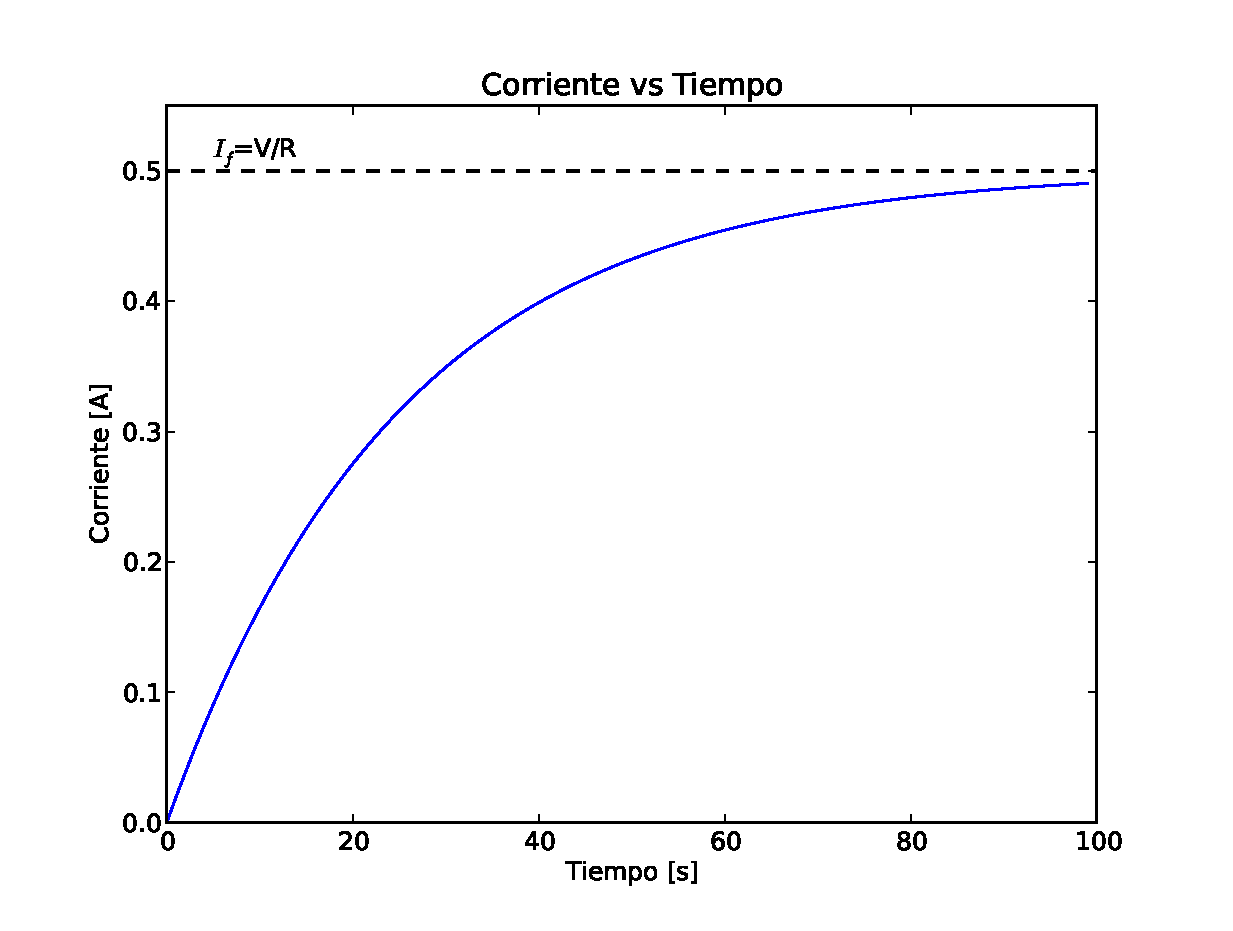
\includegraphics[scale=0.4]{RK2circuito.eps} 
\end{figure}
\end{frame}
\begin{frame}[fragile]
\fontsize{10}{10}\selectfont
\begin{lstlisting}
from numpy import *
import matplotlib.pyplot as plt

L=50.0
R=20.0
V=10.0
h=0.1
corriente=0
I=[]
I.append(0)

for i in range(99):
    k1=h*((-R/L)*corriente+(V/L))
    k2=h*((-R/L)*(corriente+k1)+(V/L))
    corriente=corriente+(k1+k2)*0.5
    I.append(corriente)
\end{lstlisting}
\end{frame}
\begin{frame}
La rutina para la gráfica con \texttt{matplotlib} la pueden implementar sin mayor problema.
\\
\bigskip
Nótese que el valor de corriente límite corresponde a $I_{f}=V/R$ que alcanzaría en un tiempo mucho mayor.
\end{frame}
\end{document}